\documentclass[12pt]{article}
\usepackage{times} 			% use Times New Roman font

\usepackage[margin=1in]{geometry}   % sets 1 inch margins on all sides
\usepackage{hyperref}               % for URL formatting
\usepackage[pdftex]{graphicx}       % So includegraphics will work
\setlength{\parskip}{1em}           % skip 1em between paragraphs
\usepackage{indentfirst}            % indent the first line of each paragraph
\usepackage{datetime}
\usepackage[small, bf]{caption}
\usepackage{listings}               % for code listings
\usepackage{xcolor}                 % for styling code
\usepackage{multirow}

%New colors defined below
\definecolor{backcolour}{RGB}{246, 246, 246}   % 0xF6, 0xF6, 0xF6
\definecolor{codegreen}{RGB}{16, 124, 2}       % 0x10, 0x7C, 0x02
\definecolor{codepurple}{RGB}{170, 0, 217}     % 0xAA, 0x00, 0xD9
\definecolor{codered}{RGB}{154, 0, 18}         % 0x9A, 0x00, 0x12

%Code listing style named "gcolabstyle" - matches Google Colab
\lstdefinestyle{gcolabstyle}{
  basicstyle=\ttfamily\small,
  backgroundcolor=\color{backcolour},   
  commentstyle=\itshape\color{codegreen},
  keywordstyle=\color{codepurple},
  stringstyle=\color{codered},
  numberstyle=\ttfamily\footnotesize\color{darkgray}, 
  breakatwhitespace=false,         
  breaklines=true,                 
  captionpos=b,                    
  keepspaces=true,                 
  numbers=left,                    
  numbersep=5pt,                  
  showspaces=false,                
  showstringspaces=false,
  showtabs=false,                  
  tabsize=2
}

\lstset{style=gcolabstyle}      %set gcolabstyle code listing

% to make long URIs break nicely
\makeatletter
\g@addto@macro{\UrlBreaks}{\UrlOrds}
\makeatother

% for fancy page headings
\usepackage{fancyhdr}
\setlength{\headheight}{13.6pt} % to remove fancyhdr warning
\pagestyle{fancy}
\fancyhf{}
\rhead{\small \thepage}
\lhead{\small HW\#, LAST NAME}  % EDIT THIS, REPLACE # with HW number
\chead{\small CS 532, Fall 2020} 

%-------------------------------------------------------------------------
\begin{document}

\begin{centering}
{\large\textbf{HW\# - CS723}}\\ % EDIT THIS
                                % REPLACE # with HW num and ADD title
YOUR NAME\\                     % EDIT THIS
DUE DATE\\                      % EDIT THIS
\end{centering}

%-------------------------------------------------------------------------

% The * after \section just says to not number the sections
\section*{Overview}

\emph{For our solution to the problem of 3D point-set alignment, we provide an implementation of the Iterative Closest Point (ICP) algorithm for 3D point alignment.  Our program, when run, will take in two helix-axis protein database (PDB) files, convert the residue coordinates to 3-D points and calculate the transformation matrix to transform one PCB into another.  Our program works on any PCD but results are strongest when the two PCD's are transformations (similar geometry) of one another or are helix axis.  To accommodate point set's of varying sizes, we have provided a filtering mechanism to pass through the denser of the two point clouds and remove points so that they are of equal size.  These points are not removed from the resulting transformed PDB's, only the array of 3-D points used to generate a transform.  Our program utilizes Biopython module in python3 to programmatically alter the coordinates associated with each residue in the original PDB. This parameters provided to the ICP were chosen from testing and remain optimized. As the results show below, the registration of helices and helix-axis are both strong and optimization could stand to render even tighter alignments.  The program could be extended for full automated alignment of helices if a solution to compute helix axis' was provided to feed the axis' into the algorithm.\newline\newline NOTE: 
Please visit: \url{https://colab.research.google.com/drive/1IYXW43aQeekV1W7goZX8XrZkBU4yzGAI?usp=sharing} where a helix-axis transformation along with the required modules are included for ease-of-viewing along with further instructions and code explanations.}

\subsection*{Implementation Details}

\emph{Below are the three methods used to calculate the best transformation matrix for two sets of 3-D points.  This algorithm is agnostic to PCD's and takes two numpy arrays of 3-D points, A and B, to use in the transformation.  A catching mechanism was put in for 3-D points of unequal lengths as can be seen on line 79.  We filter the 3-D points to be of equal length prior to using icp. The Iterative Closest Point method finds best-fit transform that maps points A on to points B. The  final homogeneous transformation that maps A on to B is found using Euclidean Distances for localization of points in conjunction with the k- nearest neighbors method.  The knn method finds the nearest euclidean neighbor in dst for each point in src. \newline\newline As can be seen in the Driver method beginning on line 264, the two helix-axis PDB's are passed to the method PDBToNpy which convert the 3-D coordinates associated with each residue.  These numpy arrays are used as the agnostic 3-D point arrays which icp requires and it is on these that we filter out points and account for mismatches in size.  The two numpy arrays are then passed into the method TransformAllPoints which facilitates the prepossessing of the numpy arrays and the hand off to the icp method.  What is returned into t3 on line 268 is a 4-D matrix consisting of the transformation and rotation matrices.  We use this transformation matrix to transform the points using numpy in the CreatePDB method.  This method also composes a BioPython structure with the new coordinate transformations and outputs a transformed PDB file that can be loaded into chimera or any desired visualization software.  After performing the transformation matrix and transforming the helix axis', the program allows for the optional input of the two helix files corresponding to the two helix axis'.  Using the transformation matrix applied in the prior steps, it will transform the points of the helix file and output a transformed helix in the same fashion as is done with the axis.  }

%Importing code from file
\lstinputlisting[language=Python, caption=Python sample code loaded from file, label=lst:import]{ICPTransformation.py}
\subsection*{Sample outputs}
\emph{The following is a visualization sequence of the algorithm.  The images are captured using UCSF's Chimera for protein visualization. We use helix1-axis.pdb and helix2-axis.pdb with the intent to transform helix1-axis onto helix2-axis.  Figure 1 shows the two helices in Chimera loaded with their initial residues coordinates.  Because of their relative distance, the rendered visualization is difficult to interpret and thus we drew bounding elipses around each helix-axis.  The subsequent figures show multiple views of the scene in which the transformed helix1-axis pdb was opened along with the helix2-axis.  As is demonstrated below, the icp algorithm proves to be an effective method for the alignment of two helices.  For reference, helix2-axis.pdb is shown in red and helix1-axis.pdb(transformed) is show in green.}
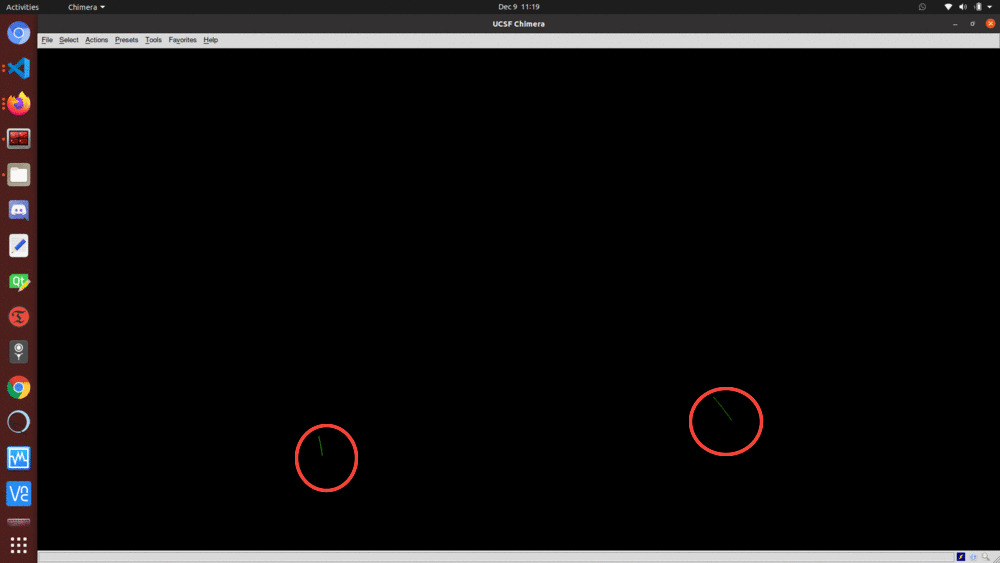
\includegraphics[trim=0 20 10 50, clip,width=\textwidth] {PreTransformBounded.jpg}
\captionof{figure}{Pre Transform.}
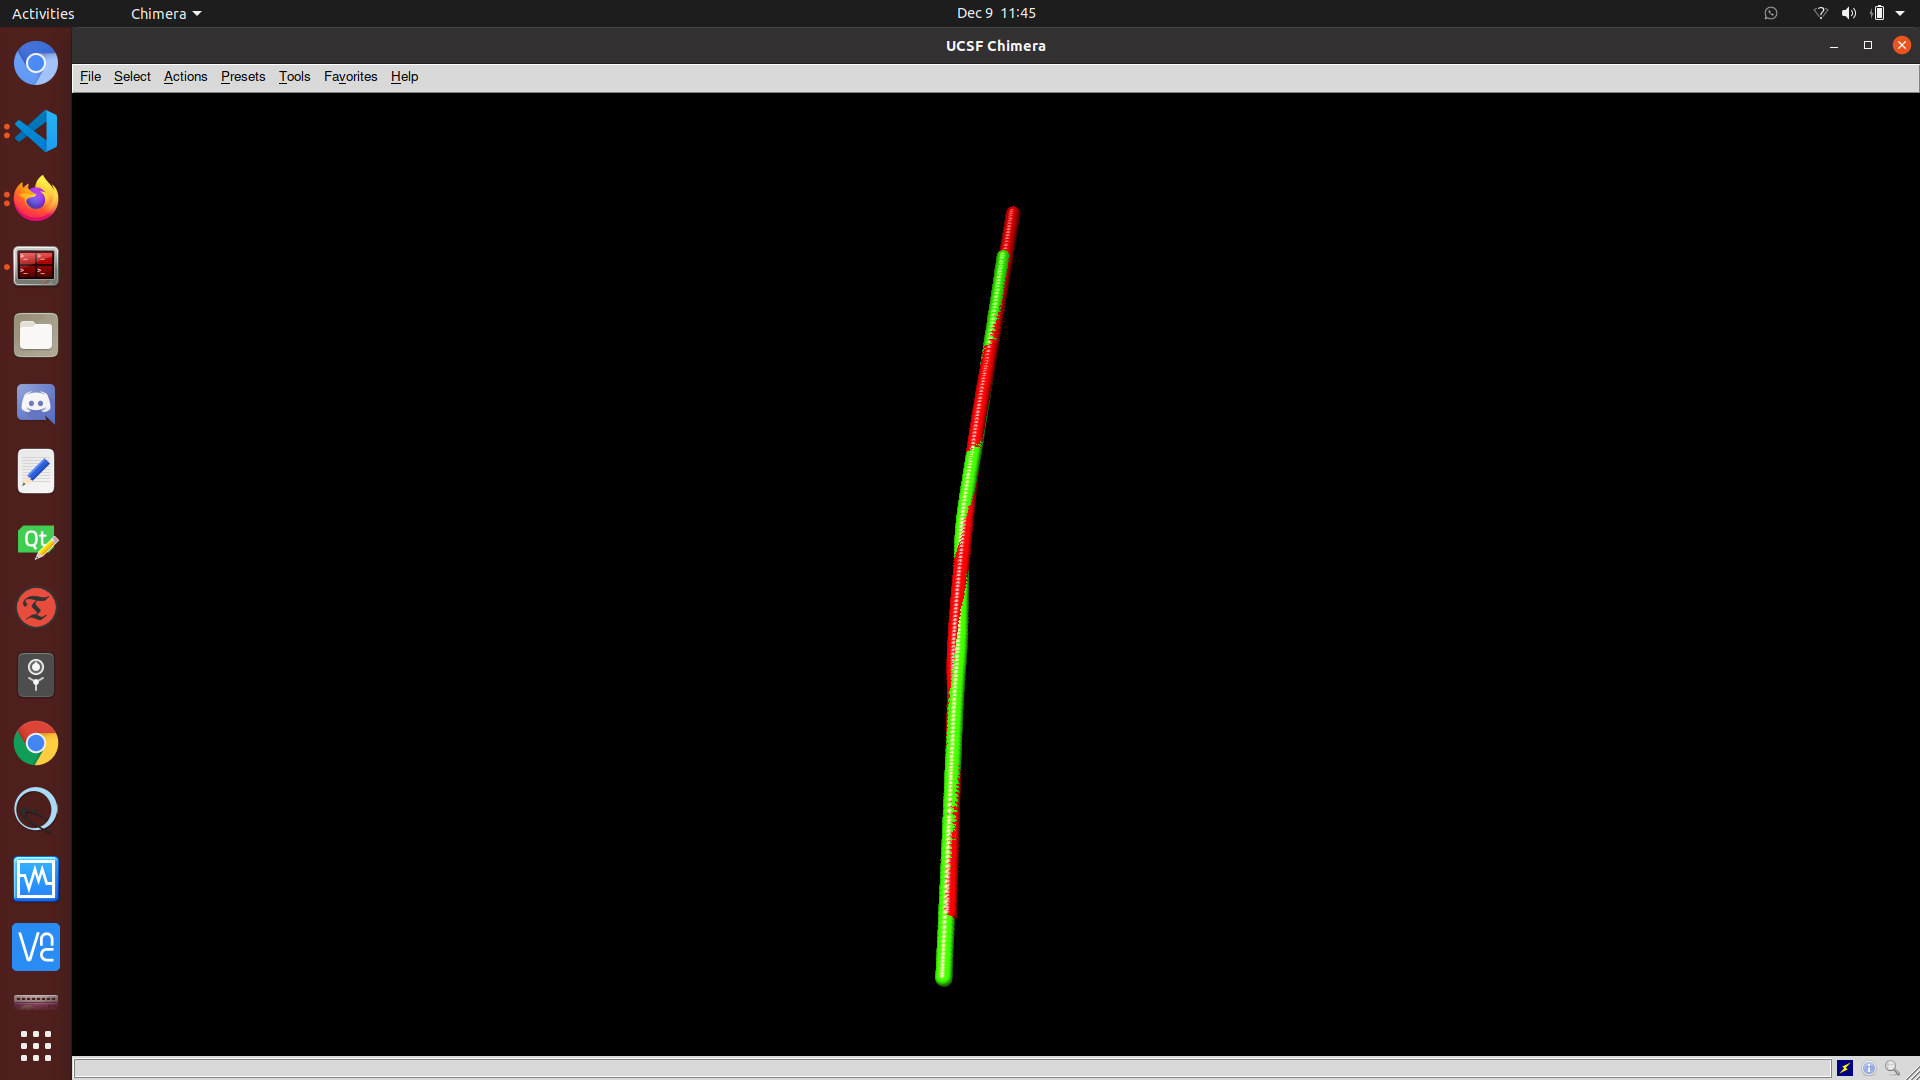
\includegraphics[trim=0 20 10 50, clip,width=\textwidth] {TopView.png}
\captionof{figure}{Top View.}
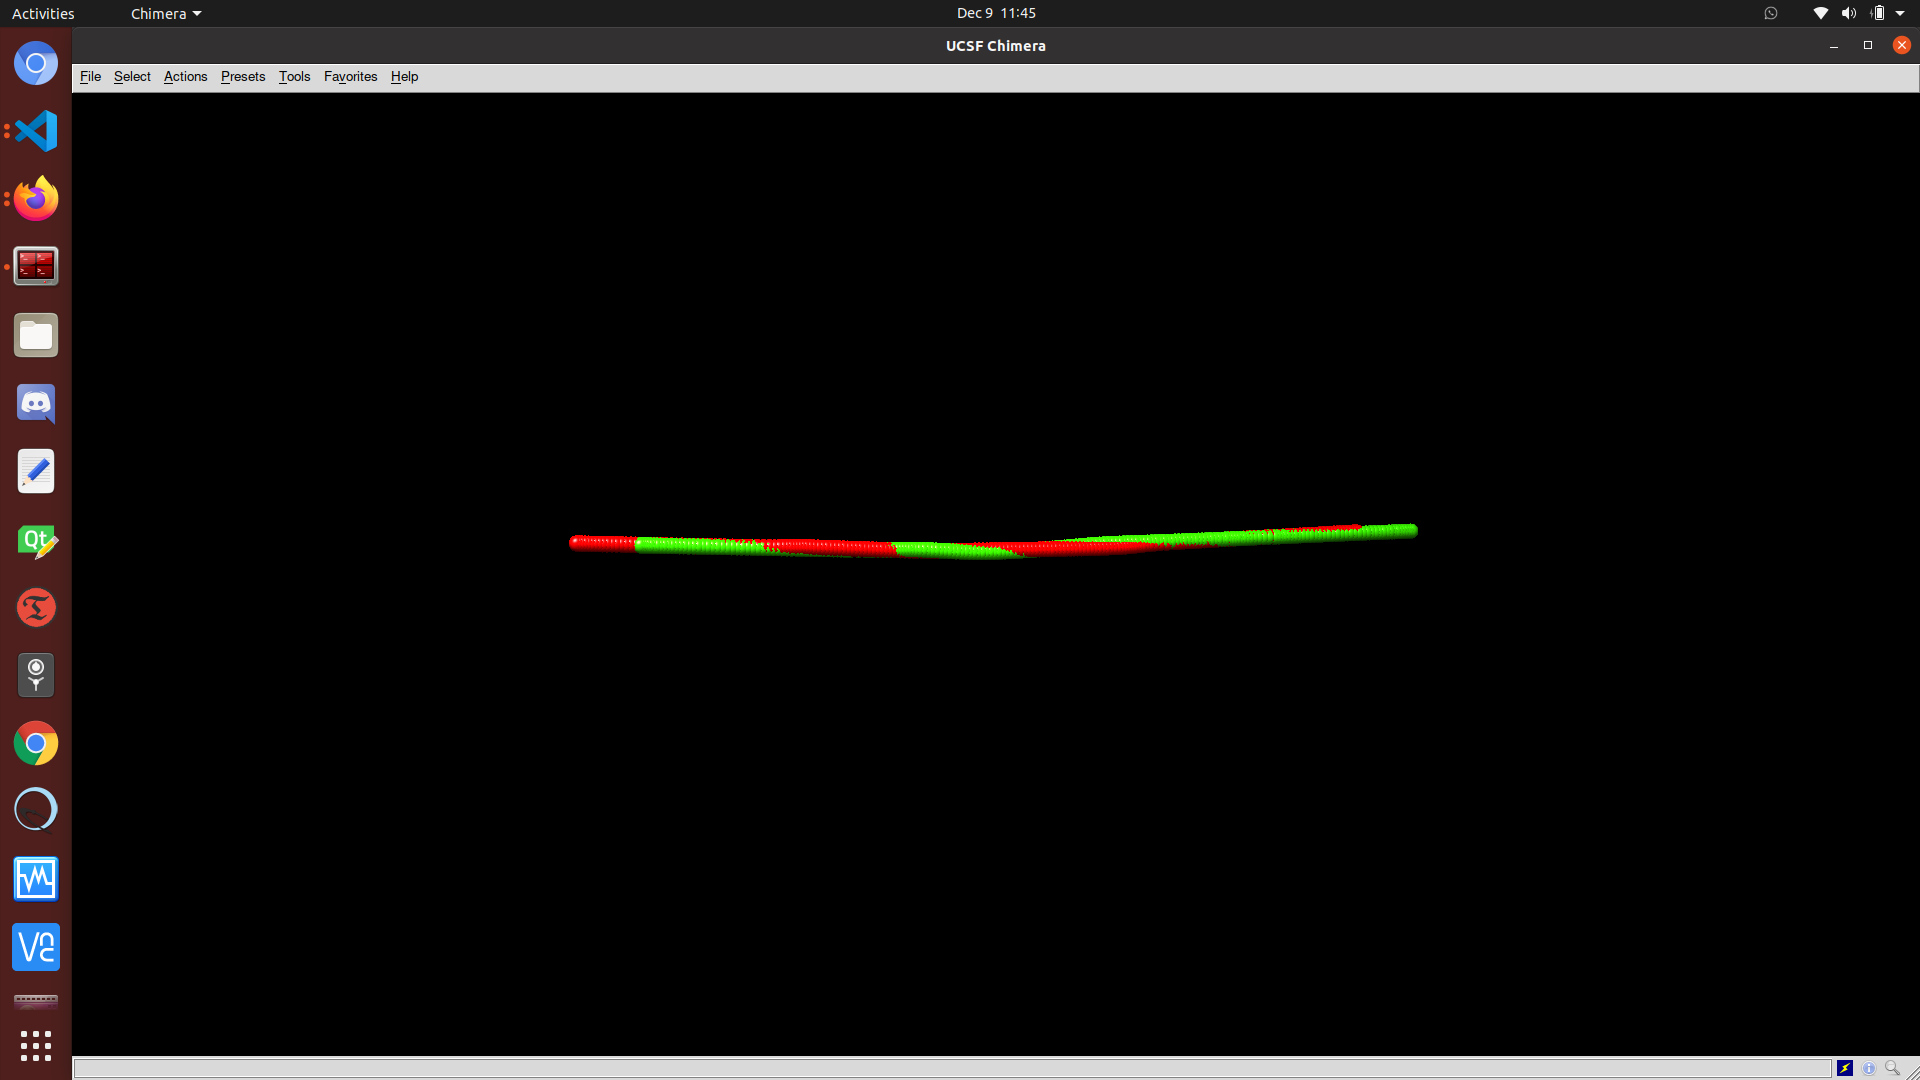
\includegraphics[trim=0 20 10 50, clip,width=\textwidth] {SideView1.png}
\captionof{figure}{Side View.}
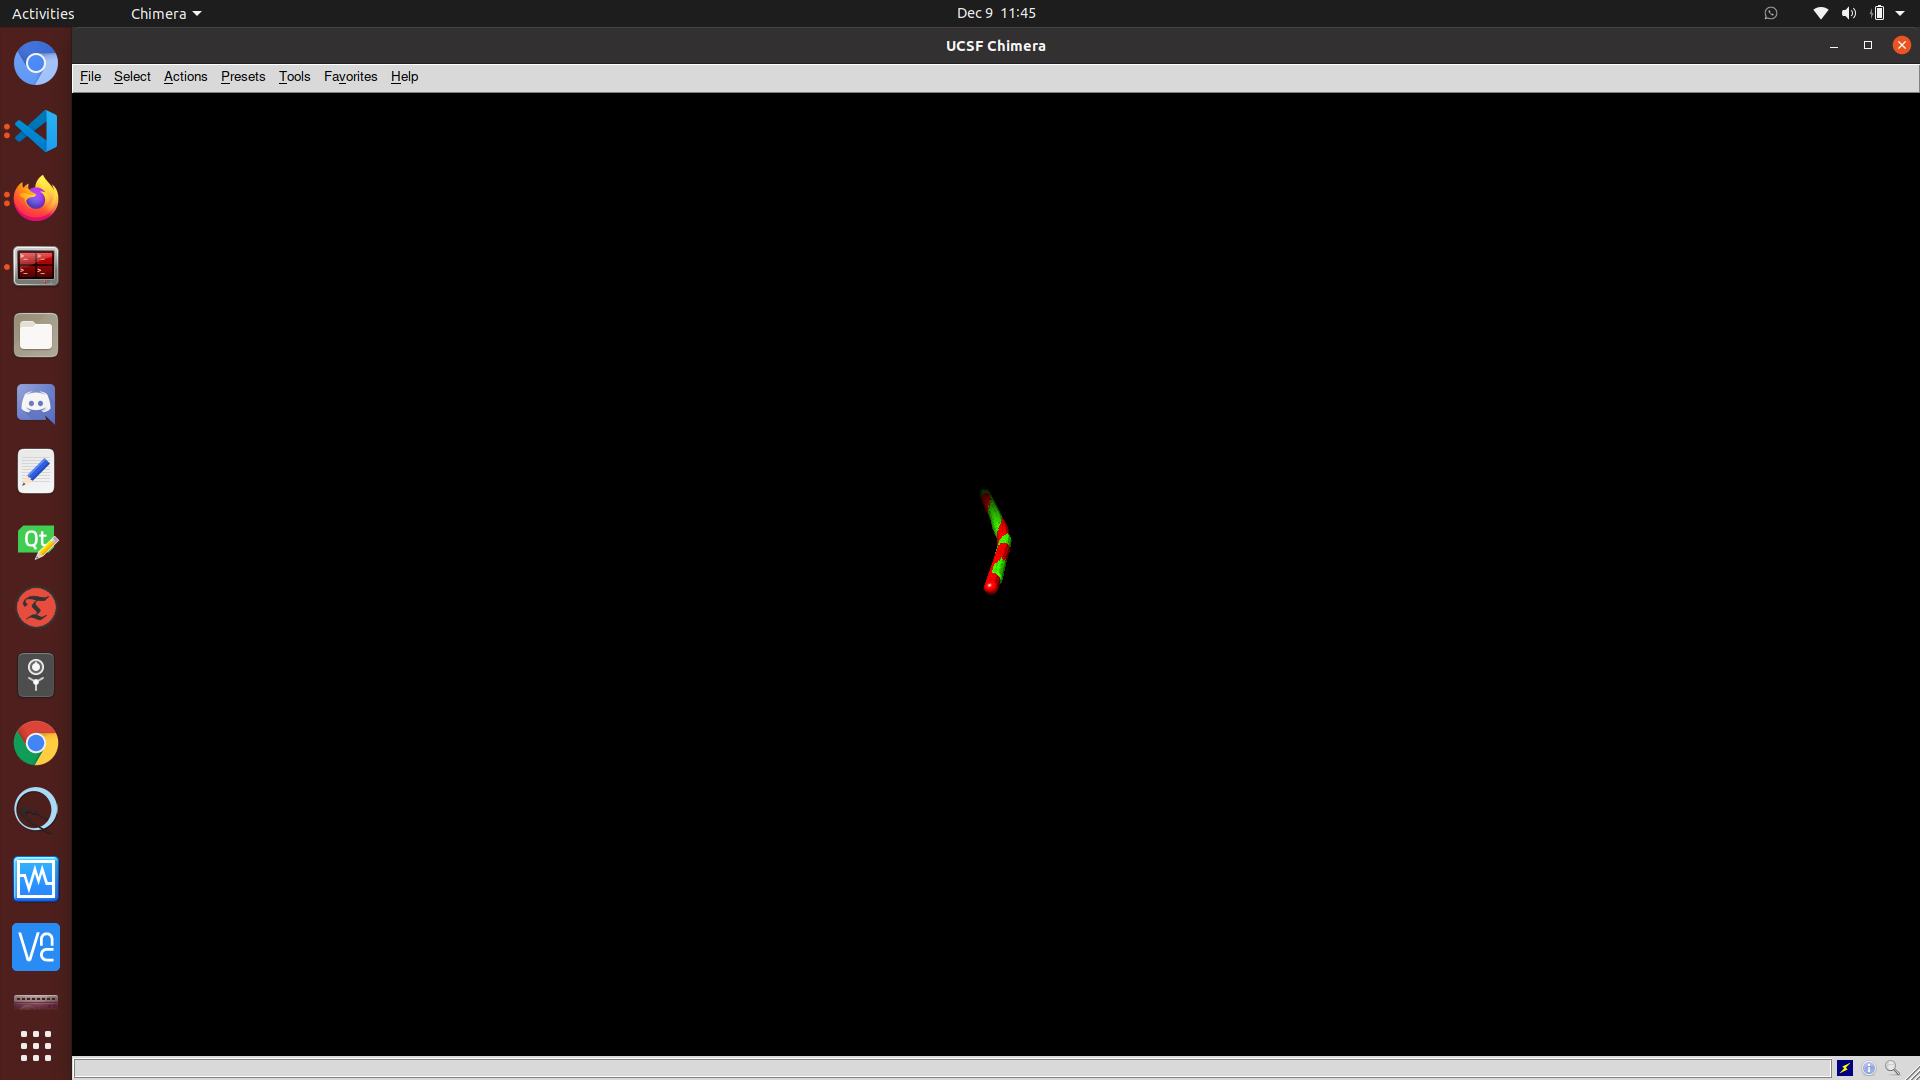
\includegraphics[trim=0 20 10 50, clip,width=\textwidth] {Front.png}
\captionof{figure}{Head-On View.}
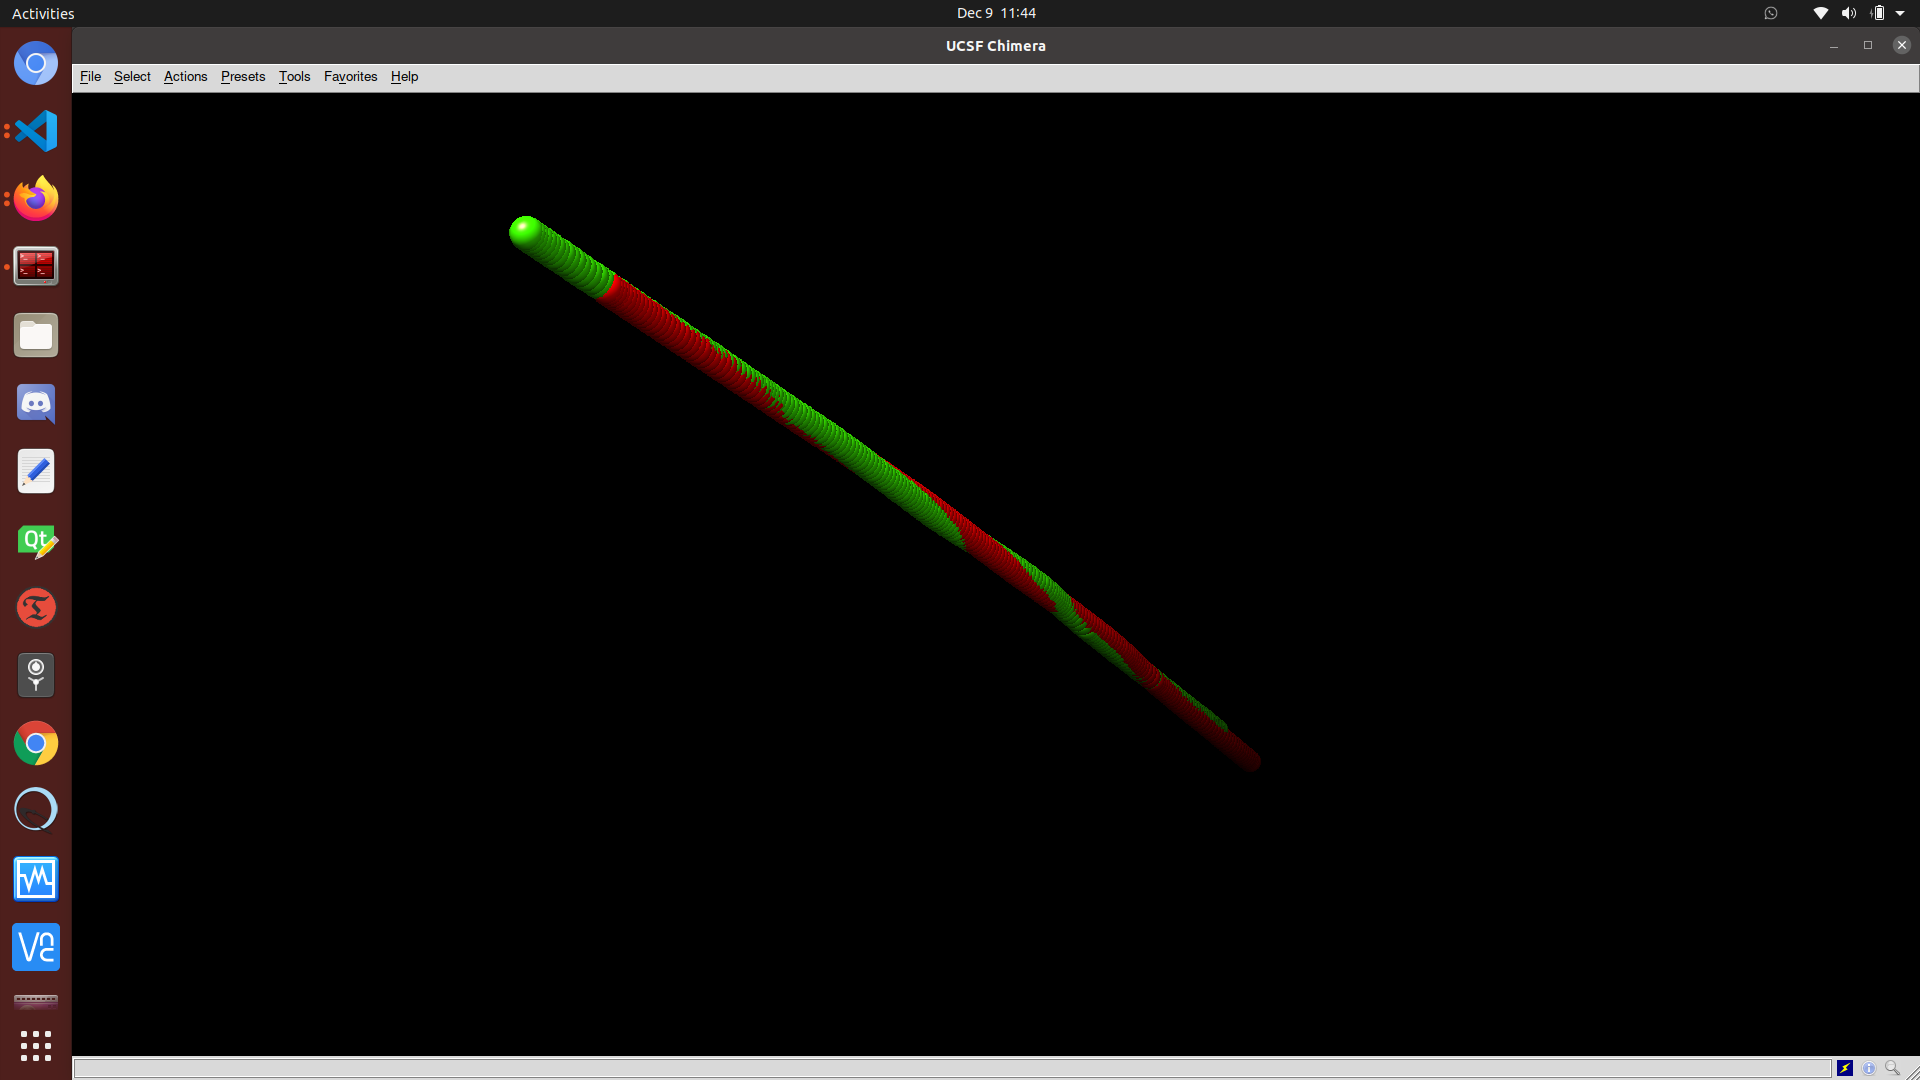
\includegraphics[trim=0 20 10 50, clip,width=\textwidth] {TopDiagonal.png}
\captionof{figure}{Diagonal View.}

\subsection*{Running instructions for helix axis transformation. (Default files.)}
\emph{\newline Please ensure the proper modules are installed, for full list and interactive demo please see: \url{https://colab.research.google.com/drive/1IYXW43aQeekV1W7goZX8XrZkBU4yzGAI?usp=sharing } where dependencies are listed in the top cell.}
\newline\newline 1) Run 'python3 ICPTransformation.py'
\newline 2) ENTER 1 to use default test cases helix1-axis.pdb and helix2-axis.pdb, included already in the folder.
\newline 3) View the transformation matrix in the terminal and helix1AxisTransform.pdb
\newline 4) If desired, open Chimera and load helix2-axis.pdb.  Then open helix1AxisTransform.pdb for visual verification.
\newline 5) In the terminal enter the helix pdb filepath associated with helix-axis1.  In this case, enter 'helix1.pdb'. This will apply the transformation matrix to each residue coordinate in helix1.pdb as it did to helix1-axis.pdb in step 2.
\newline 6) Enter 'helix1.pdb' to apply the transform to each residue coordinate in helix1.pdb.
\newline 7) The transformed helix is in fullHelix1Transformed.pdb.  Open in chimera along with helix2.pdb for viewing.

\subsection*{Running instructions for helix axis transformation. (Custom files.)}
\emph{\newline Please ensure the proper modules are installed, for full list and interactive demo please see: \url{https://colab.research.google.com/drive/1IYXW43aQeekV1W7goZX8XrZkBU4yzGAI?usp=sharing } where dependencies are listed in the top cell.}
\newline\newline 1) Run 'python3 ICPTransformation.py'
\newline 2) ENTER '2' and input the first and second helix axis files.  The first will be transformed into the second.
\newline 3) View the transformation matrix in the terminal and helix1AxisTransform.pdb
\newline 4) If desired, open Chimera and load second helix axis file entered in step 2.  Then open helix1AxisTransform.pdb for visual verification of the transformation.
\newline 5) In the terminal enter the helix pdb filepath associated with helix-axis1.  In this case, enter 'helix1.pdb'. This will apply the transformation matrix to each residue coordinate in helix1.pdb as it did to helix1-axis.pdb in step 2.
\newline 6) Enter the file path of the helix associated with helix axis 1 from step 2 to apply the transform to each residue coordinate in the full helix file.
\newline 7) The transformed helix is in fullHelix1Transformed.pdb.  Open in chimera along with helix2.pdb for viewing. \newline\newline NOTE: The two files fullHelix1Transformed.pdb and helix1AxisTransform.pdb are overwritten each run.

\section*{References}

\begin{itemize}
    \item {GitHub, \url{https://github.com/rmslick/HelixAxisRegistration.git}}
    \item {Colab, \url{https://colab.research.google.com/drive/1IYXW43aQeekV1W7goZX8XrZkBU4yzGAI?usp=sharing}}
\end{itemize}

\end{document}

